\PassOptionsToPackage{unicode}{hyperref}
\documentclass[aspectratio=1610, 11pt]{beamer}

\usepackage{amsmath}
\usepackage{amssymb}
\usetheme{tudo}

\title{Datenstrukturen, Algorithmen und Prorammierung~2}
\author[A.~Coja-Oghlan]{Amin Coja-Oghlan}
\institute[DAP2]{Lehrstuhl Informatik 2\\Fakult\"at f\"ur Informatik}

\newcommand\dist{\mathrm{dist}}
\renewcommand{\vec}[1]{\boldsymbol{#1}}
\newcommand\NULL{{\tt NULL}}
\newcommand\dd{\mathrm d}
\newcommand\eul{\mathrm e}
\newcommand\cA{\mathcal A}
\newcommand\cB{\mathcal B}
\newcommand\cC{\mathcal C}
\newcommand\cD{\mathcal D}
\newcommand\cE{\mathcal E}
\newcommand\cF{\mathcal F}
\newcommand\cG{\mathcal G}
\newcommand\cH{\mathcal H}
\newcommand\cI{\mathcal I}
\newcommand\cJ{\mathcal J}
\newcommand\cK{\mathcal K}
\newcommand\cL{\mathcal L}
\newcommand\cM{\mathcal M}
\newcommand\cN{\mathcal N}
\newcommand\cO{\mathcal O}
\newcommand\cP{\mathcal P}
\newcommand\cQ{\mathcal Q}
\newcommand\cR{\mathcal R}
\newcommand\cS{\mathcal S}
\newcommand\cT{\mathcal T}
\newcommand\cU{\mathcal U}
\newcommand\cV{\mathcal V}
\newcommand\cW{\mathcal W}
\newcommand\cX{\mathcal X}
\newcommand\cY{\mathcal Y}
\newcommand\cZ{\mathcal Z}
\newcommand\fA{\mathfrak A}
\newcommand\fB{\mathfrak B}
\newcommand\fC{\mathfrak C}
\newcommand\fD{\mathfrak D}
\newcommand\fE{\mathfrak E}
\newcommand\fF{\mathfrak F}
\newcommand\fG{\mathfrak G}
\newcommand\fH{\mathfrak H}
\newcommand\fI{\mathfrak I}
\newcommand\fJ{\mathfrak J}
\newcommand\fK{\mathfrak K}
\newcommand\fL{\mathfrak L}
\newcommand\fM{\mathfrak M}
\newcommand\fN{\mathfrak N}
\newcommand\fO{\mathfrak O}
\newcommand\fP{\mathfrak P}
\newcommand\fQ{\mathfrak Q}
\newcommand\fR{\mathfrak R}
\newcommand\fS{\mathfrak S}
\newcommand\fT{\mathfrak T}
\newcommand\fU{\mathfrak U}
\newcommand\fV{\mathfrak V}
\newcommand\fW{\mathfrak W}
\newcommand\fX{\mathfrak X}
\newcommand\fY{\mathfrak Y}
\newcommand\fZ{\mathfrak Z}
\newcommand\fa{\mathfrak a}
\newcommand\fb{\mathfrak b}
\newcommand\fc{\mathfrak c}
\newcommand\fd{\mathfrak d}
\newcommand\fe{\mathfrak e}
\newcommand\ff{\mathfrak f}
\newcommand\fg{\mathfrak g}
\newcommand\fh{\mathfrak h}
%\newcommand\fi{\mathfrak i}
\newcommand\fj{\mathfrak j}
\newcommand\fk{\mathfrak k}
\newcommand\fl{\mathfrak l}
\newcommand\fm{\mathfrak m}
\newcommand\fn{\mathfrak n}
\newcommand\fo{\mathfrak o}
\newcommand\fp{\mathfrak p}
\newcommand\fq{\mathfrak q}
\newcommand\fr{\mathfrak r}
\newcommand\fs{\mathfrak s}
\newcommand\ft{\mathfrak t}
\newcommand\fu{\mathfrak u}
\newcommand\fv{\mathfrak v}
\newcommand\fw{\mathfrak w}
\newcommand\fx{\mathfrak x}
\newcommand\fy{\mathfrak y}
\newcommand\fz{\mathfrak z}
\newcommand\vA{\vec A}
\newcommand\vB{\vec B}
\newcommand\vC{\vec C}
\newcommand\vD{\vec D}
\newcommand\vE{\vec E}
\newcommand\vF{\vec F}
\newcommand\vG{\vec G}
\newcommand\vH{\vec H}
\newcommand\vI{\vec I}
\newcommand\vJ{\vec J}
\newcommand\vK{\vec K}
\newcommand\vL{\vec L}
\newcommand\vM{\vec M}
\newcommand\vN{\vec N}
\newcommand\vO{\vec O}
\newcommand\vP{\vec P}
\newcommand\vQ{\vec Q}
\newcommand\vR{\vec R}
\newcommand\vS{\vec S}
\newcommand\vT{\vec T}
\newcommand\vU{\vec U}
\newcommand\vV{\vec V}
\newcommand\vW{\vec W}
\newcommand\vX{\vec X}
\newcommand\vY{\vec Y}
\newcommand\vZ{\vec Z}
\newcommand\va{\vec a}
\newcommand\vb{\vec b}
\newcommand\vc{\vec c}
\newcommand\vd{\vec d}
\newcommand\ve{\vec e}
\newcommand\vf{\vec f}
\newcommand\vg{\vec g}
\newcommand\vh{\vec h}
\newcommand\vi{\vec i}
\newcommand\vj{\vec j}
\newcommand\vk{\vec k}
\newcommand\vl{\vec l}
\newcommand\vm{\vec m}
\newcommand\vn{\vec n}
\newcommand\vo{\vec o}
\newcommand\vp{\vec p}
\newcommand\vq{\vec q}
\newcommand\vr{\vec r}
\newcommand\vs{\vec s}
\newcommand\vt{\vec t}
\newcommand\vu{\vec u}
\renewcommand\vv{\vec v}
\newcommand\vw{\vec w}
\newcommand\vx{\vec x}
\newcommand\vy{\vec y}
\newcommand\vz{\vec z}
\renewcommand\AA{\mathbb A}
\newcommand\NN{\mathbb N}
\newcommand\ZZ{\mathbb Z}
\newcommand\PP{\mathbb P}
\newcommand\QQ{\mathbb Q}
\newcommand\RR{\mathbb R}
\newcommand\RRpos{\mathbb R_{\geq0}}
\renewcommand\SS{\mathbb S}
\newcommand\CC{\mathbb C}
\newcommand{\ord}{\mathrm{ord}}
\newcommand{\id}{\mathrm{id}}
\newcommand{\pr}{\mathrm{P}}
\newcommand{\Vol}{\mathrm{vol}}
\newcommand\norm[1]{\left\|{#1}\right\|} 
\newcommand\sign{\mathrm{sign}}
\newcommand{\eps}{\varepsilon}
\newcommand{\abs}[1]{\left|#1\right|}
\newcommand\bc[1]{\left({#1}\right)} 
\newcommand\cbc[1]{\left\{{#1}\right\}} 
\newcommand\bcfr[2]{\bc{\frac{#1}{#2}}} 
\newcommand{\bck}[1]{\left\langle{#1}\right\rangle} 
\newcommand\brk[1]{\left\lbrack{#1}\right\rbrack} 
\newcommand\scal[2]{\bck{{#1},{#2}}} 
\newcommand{\vecone}{\mathbb{1}}
\newcommand{\tensor}{\otimes}
\newcommand{\diag}{\mathrm{diag}}
\newcommand{\ggt}{\mathrm{ggT}}
\newcommand{\kgv}{\mathrm{kgV}}
\newcommand{\trans}{\top}
\newcommand{\Karonski}{Karo\'nski}
\newcommand{\Erdos}{Erd\H{o}s}
\newcommand{\Renyi}{R\'enyi}
\newcommand{\Lovasz}{Lov\'asz}
\newcommand{\Juhasz}{Juh\'asz}
\newcommand{\Bollobas}{Bollob\'as}
\newcommand{\Furedi}{F\"uredi}
\newcommand{\Komlos}{Koml\'os}
\newcommand{\Luczak}{\L uczak}
\newcommand{\Kucera}{Ku\v{c}era}
\newcommand{\Szemeredi}{Szemer\'edi}

\newcommand{\mytitle}{K\"urzstes Pfade}

\begin{document}

\frame[plain]{\titlepage}

\begin{frame}\frametitle{\mytitle}
	\begin{exampleblock}{Worum geht es?}
		\begin{itemize}
			\item wir lernen den Dijkstra-Algorithmus f\"ur k\"urzeste Pfade kennen
			\item mittels priority queues kann Dijkstra effizient implementiert  werden
			\item wir lernen einen exakten Algorithmus f\"ur das Travelling Salesman-Problem kennen
		\end{itemize}
	\end{exampleblock}
\end{frame}

\begin{frame}\frametitle{\mytitle}
	\begin{block}{Das k\"urzeste-Pfade-Problem}
 		\begin{itemize}
			\item gegeben ist ein \emph{gewichteter} Graph $G,c$
			\item das bedeutet, da\ss\ $c:E(G)\to\QQ_{\geq0}$ \hfill[``Kosten'' oder ``L\"ange'' einer Kante]
			\item ferner sind zwei Knoten $s,t$ gegeben
			\item das Ziel ist, einen k\"urzesten Pfad von $s$ nach $t$ zu finden
			\item die \alert{L\"ange} des Pfades $p=(v_0,\ldots,v_\ell)$ ist dabei definiert als
				\begin{align*}
					c(p)=\sum_{i=1}^\ell c(v_{i-1}v_i)
				\end{align*}
		\end{itemize}
	\end{block}
\end{frame}

\begin{frame}\frametitle{\mytitle}
	\begin{overprint}
		\onslide<1>
\begin{exampleblock}{Der Dijkstra-Algorithmus}
		\begin{itemize}
			\item der Dijkstra-Algorithmus basiert auf dem Paradigma der \emph{dynamischen Programmierung}
			\item der Algorithmus baut aus L\"osungen kleinerer Teilprobleme die L\"osungen immer gr\"o\ss erer Teilprobleme zusammen, bis schlie\ss lich das Gesamtproblem gel\"ost ist
			\item im Fall des k\"urzesten-Pfade-Problems liegt die Beobachtung zugrunde, da\ss\ ein k\"urzester Pfad von $s$ nach $t$ aus k\"urzesten Teilpfaden besteht
		\end{itemize}
	\end{exampleblock}
		\onslide<2>
\begin{exampleblock}{Algorithmus Dijkstra}
		\begin{enumerate}
			\item F\"ur alle $v\in V(G)$ setze $\delta(v)=\infty$ und $p(v)=\emptyset$.
			\item Setze $\delta(s)=0$, $p(s)=s$, $S=\emptyset$ und $U=\{s\}$
			\item Solange $U\neq\emptyset$
			\item $\quad$finde $u\in U$ mit $\delta(u)=\min_{v\in U}\delta(v)$
			\item $\quad$entferne $u$ aus $U$ und f\"uge $u$ zu $S$ hinzu
			\item $\quad$f\"ur alle $w\in\partial u\setminus S$\\
			\item $\qquad$f\"uge $w$ zu $U$ hinzu
			\item $\qquad$falls $\delta(w)>\delta(u)+c(uw)$
			\item $\qquad\quad$setze $\delta(w)=\delta(u)+c(uw)$ und $p(w)=u$
			\item Gib $p,\delta$ aus
		\end{enumerate}
	\end{exampleblock}
	\end{overprint}
\end{frame}

\begin{frame}\frametitle{\mytitle}
	\begin{overprint}
		\onslide<1> \hfill\includegraphics[height=30mm]{images/dij1.pdf}	
		\onslide<2> \hfill\includegraphics[height=30mm]{images/dij2.pdf}	
		\onslide<3> \hfill\includegraphics[height=30mm]{images/dij3.pdf}	
		\onslide<4> \hfill\includegraphics[height=30mm]{images/dij4.pdf}	
		\onslide<5> \hfill\includegraphics[height=30mm]{images/dij5.pdf}	
	\end{overprint}
	\begin{exampleblock}{Beispiel}
		\begin{itemize}
			\item in jeder Iteration der Hauptschleife wird der Abstand eines Knotens von $s$ bestimmt
			\item die Abst\"ande der Nachbarn werden ggf.\ verringert
		\end{itemize}
		\end{exampleblock}
\end{frame}

\begin{frame}\frametitle{\mytitle}
	\begin{block}{Satz}
		Angenommen $G,c$ ist ein zusammenh\"angender gewichteter Graph, $s\in V(G)$ und $\delta,p$ ist die Ausgabe von Dijkstra.
		\begin{itemize}
			\item die Laufzeit betr\"agt $O(|V|^2)$
			\item f\"ur jeden Knoten $v\in V(G)$ ist $\delta(v)$ der gewichtete Abstand von $s$ nach $v$ und
				\begin{align*}
					v,p(v),\ldots,p^\ell(v)&\mbox{ mit }\ell=\min_{j\geq0}p^j(v)=s
				\end{align*}
				ist ein k\"urzester Pfad
		\end{itemize}
	\end{block}
\end{frame}

\begin{frame}\frametitle{\mytitle}
	\begin{overprint}
		\onslide<1>
		\begin{exampleblock}{Beweis: Laufzeit}
			\begin{itemize}
				\item die Hauptschleife wird $|V|$ mal durchlaufen
				\item die Berechnung von $u$ ben\"otigt Zeit $O(|V|)$
				\item anschlie\ss end werden die $O(|V|)$ Nachbarn von $u$ bearbeitet
			\end{itemize}
		\end{exampleblock}
		\onslide<2>
		\begin{exampleblock}{Beweis: Korrektheit}
			\begin{itemize}
				\item nach dem ersten Durchlauf der Hauptschleife gilt
					\begin{align*}
						U&=\partial s&S&=\cbc s\\\delta(s)&=0&\delta(v)&=c(sv)\quad(v\in\partial s)
					\end{align*}
			\end{itemize}
		\end{exampleblock}
		\onslide<3>
		\begin{exampleblock}{Beweis: Korrektheit (fortgesetzt)}
			\begin{itemize}
				\item wir beweisen, da\ss\ forthin die folgenden drei Bedingungen erf\"ullt bleiben: 
					\begin{enumerate}[(i)]
						\item $U=\partial S\setminus S$
						\item f\"ur alle $v\in S$ ist $\delta(v)$ der Abstand von $s$ nach $v$ und
							\begin{align*}
								v,p(v),\ldots,p^\ell(v)&\mbox{ mit }\ell=\min_{j\geq0}p^j(v)=s
							\end{align*}
							ist ein entsprechender k\"urzester Pfad
						\item f\"ur alle $v\in U$ ist $\delta(v)$ der Abstand von $s$ nach $v$ in $G[S\cup\cbc v]$ und \begin{align*}
								v,p(v),\ldots,p^\ell(v)&\mbox{ mit }\ell=\min_{j\geq0}p^j(v)=s
							\end{align*}
							ein entsprechender Pfad.
					\end{enumerate}
			\end{itemize}
		\end{exampleblock}
		\onslide<4>
		\begin{exampleblock}{Beweis: Korrektheit (fortgesetzt)}
			\begin{itemize}
				\item dazu f\"uhren wir Induktion nach der Anzahl der Iterationen der Hauptschleife
				\item f\"ur die erste Iteration ist nichts zu zeigen
				\item betrachte nun den n\"achsten Knoten $u$
				\item dieser erf\"ullt $\delta(u)=\min_{v\in U}\delta(v)$
				\item aus der Induktionsannahme und der Konstruktion in Schritten 5--10 folgt die Aussage (i) unmittelbar
			\end{itemize}
		\end{exampleblock}
		\onslide<5>
		\begin{exampleblock}{Beweis: Korrektheit (fortgesetzt)}
			\begin{itemize}
				\item zu Aussage (ii): nach Induktion ist $P=u,p(u),\ldots,p^\ell(u)$ mit $\ell$ minimal, so da\ss\ $p^\ell(u)=s$, ein k\"urzester Pfad von $s$ nach $u$ in $G[S\cup\cbc u]$
				\item angenommen es g\"abe in $G$ einen k\"urzeren Pfad $Q$ von $s$ nach $u$
				\item sei $z$ der erste Knoten von $Q$, der nicht in $S\cup\cbc u$ liegt
				\item dann gilt $\delta(z)\geq\delta(u)$
				\item aus der Wahl von $z$ und der Induktionsannahme folgt also
					\begin{align*}
						c(Q)\geq\delta(z)\geq\delta(u)=c(P)
					\end{align*}
				\item Widerspruch zur Annahme
			\end{itemize}
		\end{exampleblock}
		\onslide<6>
		\begin{exampleblock}{Beweis: Korrektheit (fortgesetzt)}
			\begin{itemize}
				\item die Aussage (iii) folgt aus der Aussage (ii) und der Tatsache, da\ss\ f\"ur $w\in S$ ein k\"urzester Pfad von $s$ nach $w$ in $G$ auch ein k\"urzester Pfad von $s$ nach $w$ in $G[S]$ ist
				\item da f\"ur einen zusammenh\"angenden Graphen jeder Knoten in $U$ und in der Folge in $S$ eingef\"ugt wird, folgt die Behauptung
			\end{itemize}
		\end{exampleblock}
	\end{overprint}
\end{frame}

\begin{frame}\frametitle{\mytitle}
	\begin{overprint}
		\onslide<1>
		\begin{exampleblock}{Implementierung mit priority queues}
			\begin{itemize}
				\item in Anwendungen treten h\"aufig {\em d\"unne} Graphen mit $o(|V(G)|^2)$ Kanten auf
				\item  nicht selten ist sogar $|E(G)|=O(|V(G)|)$
				\item f\"ur d\"unne Graphen ist Dijkstra relativ langsam
				\item zeitkritisch ist die Berechnung des Minimums in Schritt 4
			\end{itemize}
		\end{exampleblock}
		\onslide<2>
		\begin{exampleblock}{Erinnerung: min priority queues}
			\begin{itemize}
				\item wir haben priority queues bereits im Zusammenhang mit Heapsort kennengelernt
				\item Operationen: {\tt Insert}, {\tt ExtractMin}, {\tt DecreaseKey}
				\item jede der Operationen hat Laufzeit $O(\log n)$
				\item \itshape dies sind genau die Operationen, die wir f\"ur Dijkstra ben\"otigen!
			\end{itemize}
		\end{exampleblock}
		\onslide<3>
		\begin{block}{Korollar}
			Unter Verwendung einer min-priority-queue hat {\tt Dijkstra} eine Laufzeit von $$O(|E(G)|\log|V(G)|)$$
		\end{block}
		\begin{exampleblock}{Bemerkung}
			Eine noch bessere Laufzeit kann mit einer ausgefeilten Datenstruktur, den {\em Fibonacci-Heaps}, erzielt werden.
			Man kommt dann auf $O(|V(G)|\log|V(G)|+|E(G)|)$.
		\end{exampleblock}
	\end{overprint}
\end{frame}

\begin{frame}\frametitle{\mytitle}
	\begin{overprint}
		\onslide<1>
		\begin{exampleblock}{Travelling salesman}
			\begin{itemize}
				\item gegeben ist ein gewichteter \emph{vollst\"andiger} Graph $G,w$ auf $n$ Knoten
				\item \emph{Ziel:} eine k\"urzeste Tour, die jeden Knoten genau einmal besucht
				\item eine \alert{Tour} ist eine bijektive Abbildung $\sigma:[n]\to V(G)$
				\item die Knoten werden also in der Reihenfolge $\sigma(1),\sigma(2),\ldots,\sigma(n),\sigma(1)$ besucht
				\item die \alert{L\"ange} einer Tour ist
					\begin{align*}
						w(\sigma)&=w(\{\sigma(1),\sigma(n)\})+\sum_{i=1}^{n-1}w(\{\sigma(i),\sigma(\{i+1\}).
						\end{align*}
				\item \itshape keine Dreiecksungleichung!
			\end{itemize}
		\end{exampleblock}
		\onslide<2>
		\begin{exampleblock}{Travelling salesman}
			\begin{itemize}
				\item 				derzeit ist kein effizienter Algorithmus f\"ur TSP bekannt\hfill[NP-schwer]
				\item ``naiver'' Algorithmus: alle Permutationen durchprobieren\dots
				\item \emph{Laufzeit:}
					\begin{align*}
						\Omega(n!)=\Omega((n/\eul)^n)=\Omega(n^{n+o(n)}).
					\end{align*}
				\item \itshape polynomieller Platzbedarf!
			\end{itemize}
		\end{exampleblock}
		\onslide<3>
		\begin{exampleblock}{Bellmann-Held-Karp-Algorithmus}
			\begin{itemize}
				\item Prinzip dynamische Programmierung
				\item w\"ahle einen beliebigen Startknoten $s\in V(G)$
				\item baue eine \alert{Tabelle} auf mit einem Eintrag f\"ur jede Teilmenge $U\subseteq V(G)\setminus\cbc s$ und jeden Knoten $u\neq s$, $u\not\in U$ \item  Eintrag $T(u,U)$ ist die L\"ange eines k\"urzesten Pfades, der in $s$ startet, alle Knoten aus $U$ besucht und in $u$ endet
				\item die L\"ange einer optimalen TSP-Tour kann leicht bestimmt werden, wenn die Tabelle bekannt ist
			\end{itemize}
		\end{exampleblock}
		\onslide<4>
		\begin{block}{Lemma}
			F\"ur alle $s\in V(G)$, $\emptyset\neq U\subseteq V(G)\setminus\cbc s$, $u\in V(G)\setminus\cbc s\cup U$ gilt
			\begin{align*}
				T(u,U)&=\min_{v\in U}T(v,U\setminus\cbc v)+w(\{u,v\}),&T(u,\emptyset)&=w(\{s,u\}).
			\end{align*}
		\end{block}
		\begin{exampleblock}{Beweis}
			Sei $v$ der letzte Knoten aus $U$, der auf einem k\"urzesten Pfad von $s$ durch alle Knoten aus $U$ nach $u$ liegt.
			Dann ist die L\"ange dieses Pfades genau $w(\{u,v\})+T(v,U\setminus\cbc v)$.
		\end{exampleblock}
		\onslide<5>
		\begin{exampleblock}{\tt BHK$(G,w)$}
			\begin{enumerate}
				\item W\"ahle einen Startknoten $s$.
				\item F\"ur alle $u\in V(G)\setminus\cbc s$ setze $T(u,\emptyset)=w(\{s,u\})$.
				\item F\"ur $N=1,\ldots,n-2$
				\item $\quad$f\"ur alle $u\in V(G)\setminus\{s\}$
				\item $\quad\quad$f\"ur alle Teilmengen $U\subseteq V(G)\setminus\{u,s\}$ mit $|U|=N$
				\item $\quad\quad\quad$setze
					\begin{align*}
						T(u,U)&=\min_{v\in U}T(v,U\setminus\cbc v)+w(\{u,v\}).
					\end{align*}
				\item Gib $\min_{u\in V(G)\setminus\cbc s}T(u,V(G)\setminus\{u,s\})+w(\{u,s\})$ aus.
			\end{enumerate}
		\end{exampleblock}
		\onslide<6>
		\begin{block}{Satz}
			{\tt BHK} berechnet in Zeit $O(2^{n+o(n)})$ die L\"ange einer optimalen TSP-Tour.
		\end{block}
		\begin{exampleblock}{Beweis}
			\begin{itemize}
				\item Korrektheit folgt aus dem Lemma
				\item Laufzeit wird dominiert durch die Schleifen (3)--(6)
				\item dort wird \"uber alle Teilmengen $U\subseteq V(G)\setminus\cbc s$ iteriert
				\item die Zahl dieser Teilmengen ist $O(2^n)$
				\item f\"ur jede Teilmenge wird wiederum \"uber $O(n^2)$ Knoten $u,v$ iteriert
			\end{itemize}
		\end{exampleblock}
	\end{overprint}
\end{frame}

\begin{frame}\frametitle{\mytitle}
	\begin{exampleblock}{Zusammenfassung}
		\begin{itemize}
			\item Dijkstra berechnet k\"urzeste gewichtete Pfade
			\item wichtig ist dabei, da\ss\ die Gewichte \emph{nicht negativ} sind! (Warum?)
			\item die ``naive'' Laufzeit ist quadratisch
			\item mit min priority queues l\"a\ss t sich die Laufzeit deutlich verbessern
			\item der Algorithmus {\tt BHK} f\"ur TSP
		\end{itemize}
	\end{exampleblock}
\end{frame}

\end{document}
